\documentclass[a4paper,11pt]{article}
\usepackage[right=1in,left=1in,top=0.7in,bottom=0.7in]{geometry}
\usepackage{lipsum}
\usepackage{graphicx}
\usepackage{float}
\usepackage{cite}
\usepackage{color}
\usepackage{caption}
% \usepackage{listings}
% \usepackage{hyperref}
% \usepackage{textgreek}

\renewcommand{\familydefault}{\sfdefault}


\begin{document}
    \begin{titlepage}
        \begin{center}
            
\includegraphics[height=7.5em]{../resources/unilogo.png}
            \vspace{6em}

            {\LARGE Laboratory Protocol} \\ 
            {\huge\bfseries Characterization of Protein Stability,\\ Catalysis and Aggregation}
            \vspace{3em}
            
            {\large\bfseries Molecular Biology and Biochemistry of Life}\\
            Winter Semester 2023-24
            \vspace{12em}

            {\bfseries Authors} \\ 
            Masine Janet Tränkner\\
            Syed Alisamar Husain
            \vspace{5em}

            {\bfseries Supervisor} \\ Dr.\ Titus M. Franzmann
        \end{center}
        
    \end{titlepage}
    \pagebreak

    \tableofcontents
    \listoffigures
    \vspace{3em}
    {\noindent\Large\bfseries Author Information \vspace{0.75em}}\\
    \noindent\large Masine Janet Tränkner\\
    {\small MSc. Computational Modelling and Simulation}\\
    {\small Matriculation Number 5186813}\\
    {\it\small masine\_janet.traenkner@mailbox.tu-dresden.de}\\\vspace{0.5em}
    
    \noindent\large Syed Alisamar Husain\\
    {\small MSc. Computational Modelling and Simulation}\\
    {\small Matriculation Number 5198172}\\
    {\it\small syed\_alisamar.husain@mailbox.tu-dresden.de}
    \pagebreak

    \section{Temperature Induced Unfolding Transitions}
        The goal in this experiment is to determine the stability of the proteins Lysozyme and BSA 
        (Bovine Serum Albumin) at different concentrations, 2.5, 5 and 10 µM, by inducing unfolding 
        transitions through temperature changes.
        We detect unfolding using Fluorescence spectroscopy by measuring emission at 
        two wavelengths, 330nm and 350nm, and we expect to see a sharp increase in the ratio
        of these emissions when the protein unfolds.

        \subsection*{Measurements}
            The temperature was increased from 25 °C to 95 °C, at a rate of 2 °C per minute,
            and corresponding fluorescence at wavelengths 350nm and 330nm was measured.

            \subsubsection*{Lysozyme - Fluorescence vs. Temperature}
                \begin{figure}[H]
                    \centering
                    \begin{tabular}{cc}
                        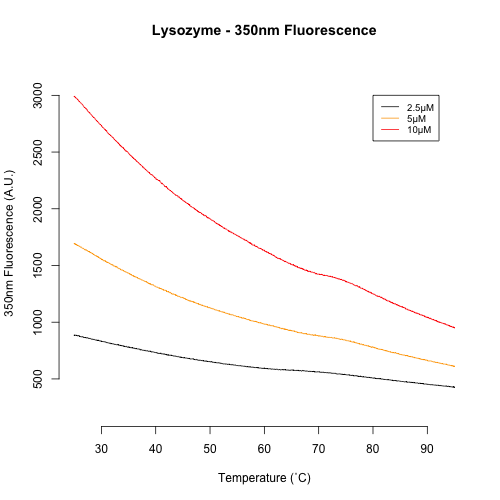
\includegraphics[width=180px]{../resources/unfolding_lys_350.png} &
                        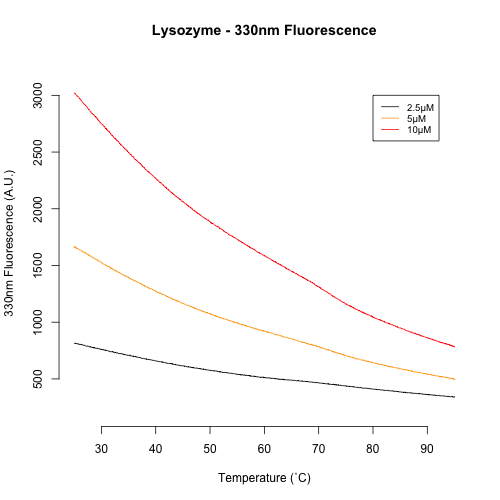
\includegraphics[width=180px]{../resources/unfolding_lys_330.png} \\
                        (a) & (b)\\
                    \end{tabular}
                    \caption{Lysozyme Fluorescence at wavelengths (a) 350nm and (b) 330nm}\label{fig:lys_flr}
                \end{figure}
                
            \subsubsection*{BSA - Fluorescence vs. Temperature}
                \begin{figure}[H]
                    \centering
                    \begin{tabular}{cc}
                        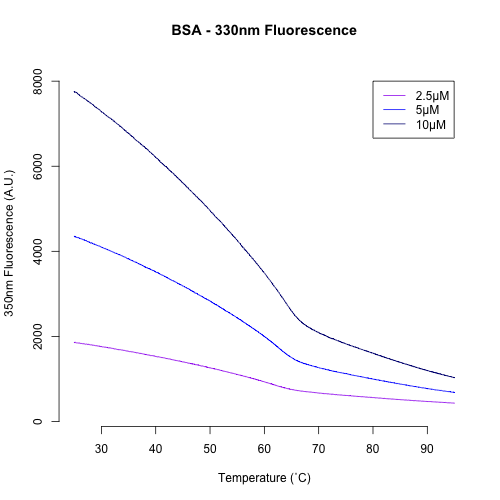
\includegraphics[width=180px]{../resources/unfolding_BSA_350.png} &
                        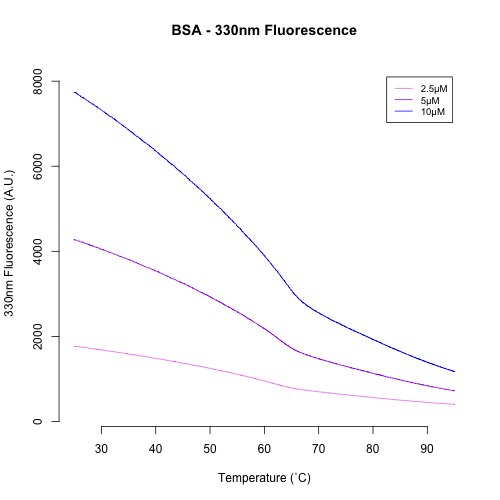
\includegraphics[width=180px]{../resources/unfolding_BSA_330.png} \\
                        (a) & (b)\\
                    \end{tabular}
                    \caption{BSA Fluorescence at wavelengths (a) 350nm and (b) 330nm}\label{fig:bsa_flr}
                \end{figure}

        \subsection*{Analysis}
            The Fluorescence Ratio graph (Figure~\ref{fig:lys_ratio} and~\ref{fig:bsa_ratio}) was used to 
            approximate the transition midpoint, while the protein's heat capacity was derived from the 
            plot's derivative. 
            Stability in the folded state arises from various interactions within the polypeptide. 
            However, upon surpassing a threshold temperature, the polypeptide 
            transitions to an unstable state. Consequently, as temperature increases, the population 
            of unfolded molecules also rises. This process behaves differently for the two proteins. 

            For Lysozyme, a low ratio can be observed at the beginning, which indicates that 
            the folded state predominates. With increasing temperature, this confirmation changes 
            up to a threshold temperature and the transition of the molecules into the unfolded state, 
            and accordingly the ratio also increases.
            \begin{figure}[H]
                \centering
                \begin{tabular}{cc}
                    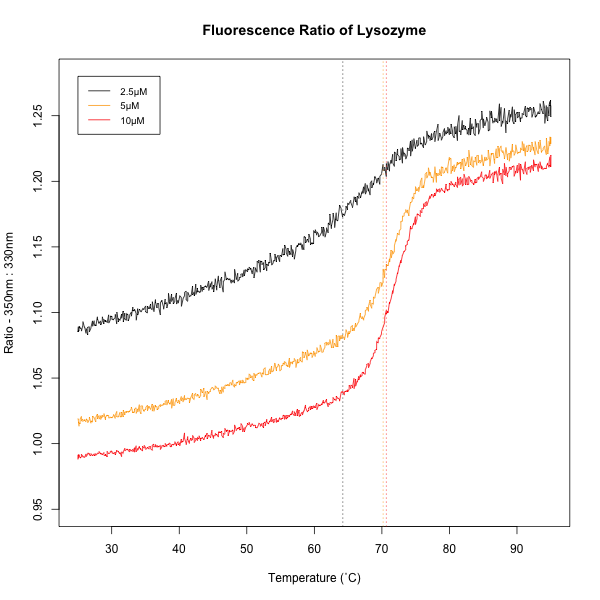
\includegraphics[width=200px]{../resources/unfolding_lys_ratio.png} &
                    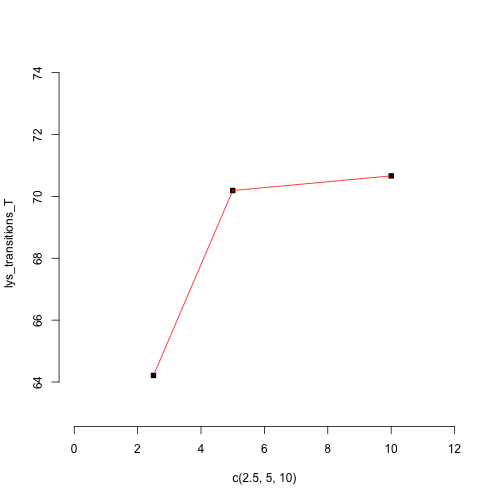
\includegraphics[width=200px]{../resources/unfolding_lys_tempVconc.png} \\
                    (a) & (b)\\
                \end{tabular}
                \caption{Ratio of Fluorescence at 350nm to 330nm for Lysozyme}
                \label{fig:lys_ratio}
            \end{figure}
            
            The opposite can be observed for BSA. Here, the ratio is already high at the start of 
            the process and falls down to a certain threshold temperature. From this point, the ratio 
            increases for all concentrations and thus also the amount of proteins in the unfolded state.
            \begin{figure}[H]
                \centering
                \begin{tabular}{cc}
                    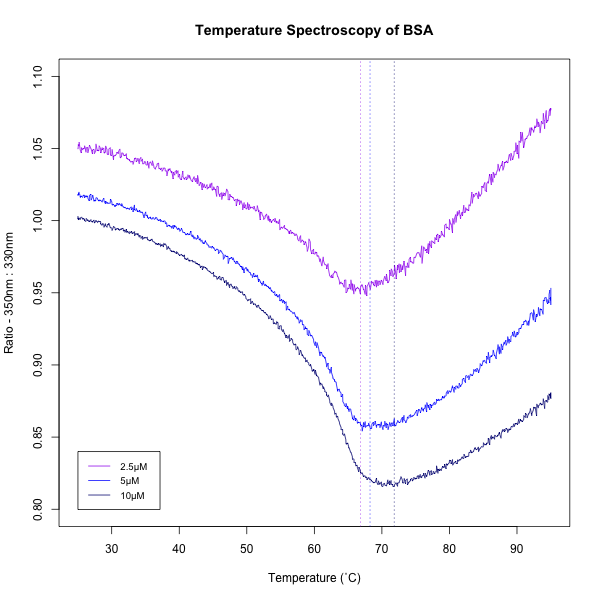
\includegraphics[width=200px]{../resources/unfolding_BSA_ratio.png} &
                    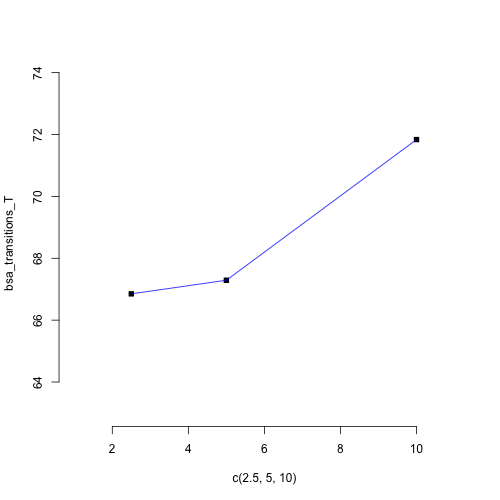
\includegraphics[width=200px]{../resources/unfolding_BSA_tempVconc.png} \\
                    (a) & (b)\\
                \end{tabular}
                \caption{Ratio of Fluorescence at 350nm to 330nm for BSA}
                \label{fig:bsa_ratio}
            \end{figure}
    \pagebreak
    
    \section{Lysozyme Aggregation}
        In this experiment, aggregation of Lysozyme was studied to understand protein aggregation, 
        where unfolded polypeptide chains of the proteins Lysozyme and Hsp26 associate irreversibly, 
        leading to the formation of large particles that scatter light. 
        Throughout the experiment, Hsp26 was used to analyze its effect on the aggregation of 
        Lysozyme with presence of TCEP.
        
        \subsection*{Measurements}
            Poor absorbance spectrometer used to do a poor-man's version of scattering. The scattering is not actually detected.
            What we do is choose a wavelength where we know nothing in the mix absorbs anything and we use that fact to say all of the intensity reduction is 
            because of the scattered light.
            \begin{figure}[H]
                \centering
                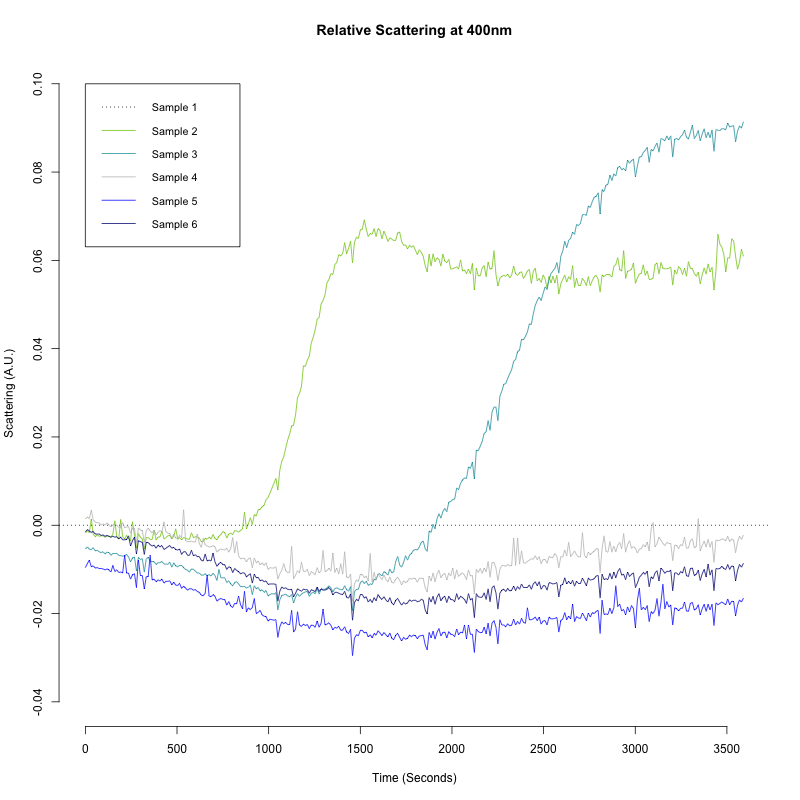
\includegraphics[width=350px]{../resources/aggregation_main.png}
                \caption{Scattering recorded as a function of time.}\label{fig:agg_main}
            \end{figure}

        \subsection*{Analysis}
            As protein aggregation increases, more light is absorbed by the sample. 
            Introducing Hsp26 into the sample solutions can regulate aggregation and, consequently, 
            absorption. At low Hsp26 concentrations (Samples 1 to 3 in Figure~\ref{fig:agg_main}), Lysozyme aggregation 
            isn't effectively inhibited. Thus, the presence of Hsp26 in the solution increases overall 
            absorption. But it can also be seen that a higher concentration of 5 µM delays the aggregation. 
            
            However, when the concentration of Hsp26 matches that of Lysozyme, aggregation is prevented, 
            resulting in lower absorbance (Sample 4). 
            The control samples lacking Lysozyme and denaturant exhibit no absorbance change at 400nm (Samples 5 and 6). 
            Only Samples 2 and 3 allow for the determination of an apparent halftime, as their curves 
            display a change of confirmation.
    \pagebreak
    
    \section{Michaelis-Menten Kinetics}
        Lactatdehydrogenase (LDH) catalyzes the reaction of the substrate pyruvate into the product, 
        lactate. In order to measure its activity, the conversion of NADH, the cofactor of LDH, NAD$^+$ 
        was observed in this experiment through spectroscopy of NADH.
        
        \subsection*{Measurements}
            \begin{figure}[H]
                \centering
                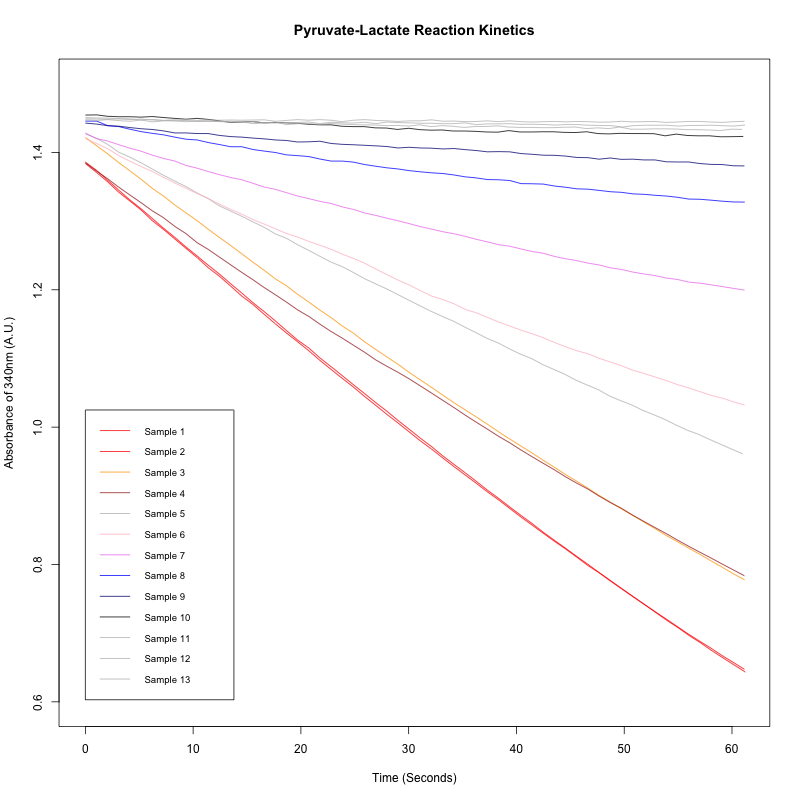
\includegraphics[width=250px]{../resources/kinetics_rates.png}
                \caption{Rates}\label{fig:mm_rates}
            \end{figure}
            
            \subsection*{Analysis}
                The Michaelis-Menten plot (see figure x left) could be plotted from the reaction rates 
                and the according concentration of substrate (NADH). It shows that for low substrate 
                concentrations, the rate of the reaction increases linearly with increasing substrate 
                concentration. As the substrate concentration increases, the rate of the reaction or 
                velocity eventually reaches a maximum value ($V_{max}$). In this region, the active sites 
                of the enzyme are largely occupied by the substrate, and the rate becomes independent 
                of further increases in substrate concentration.
            
                \begin{figure}[H]
                    \centering
                    \begin{tabular}{cc}
                        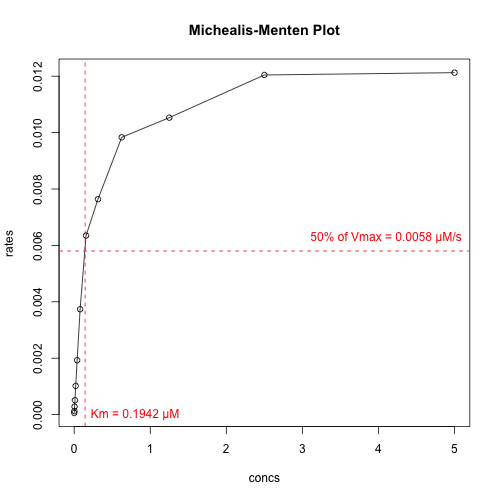
\includegraphics[width=180px]{../resources/kinetics_mmplot.png} &
                        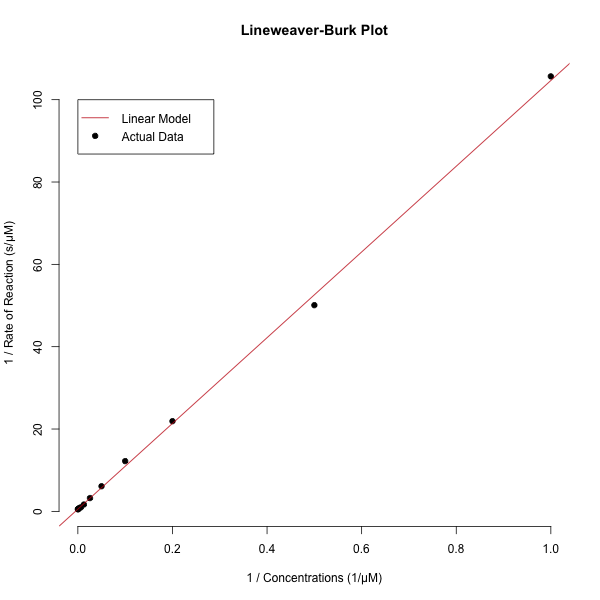
\includegraphics[width=180px]{../resources/kinetics_lbplot.png} \\
                        (a) & (b)\\
                    \end{tabular}
                    \caption{Rates}\label{fig:mm_plot}
                \end{figure}

                Derived from the Michaelis-Menten plot, the Lineweaver-Burk plot provides a linear 
                transformation. It is used for determining the kinetic constants, the maximum reaction 
                rate $V_{max}$ and the Michaelis constant $K_m$. The result for $V_{max}$ = 0.0116 µM/s and for 
                $K_m$ = 0.1942 µM, respectively.

                \begin{center}
                    \begin{tabular}{|c|}
                        \hline 
                        $V_{max}$ = 0.0116 µM/s \\
                        $K_m$ = 0.1942 µM \\
                        \hline
                    \end{tabular}
                \end{center}

    \pagebreak

    \section{UV/VIS Spectroscopy of NADH}
    Similar to the kinetics experiment, the concentration should also be measured here using UV/VIS spectroscopy.
    The detected absorbance should show local maxima for 3 specific wavelengths (208, 260 and 340 nm). It is also to be expected that the absorbance also increases with increasing NADH concentration. However, according to figure x, the absorbance increases from sample 1 to 3, then increases for the samples 4 and 5 and again increases for sample 6, without exceeding the highest absorbance of sample 2. 

        \begin{figure}[H]
            \centering
            \begin{tabular}{cc}
                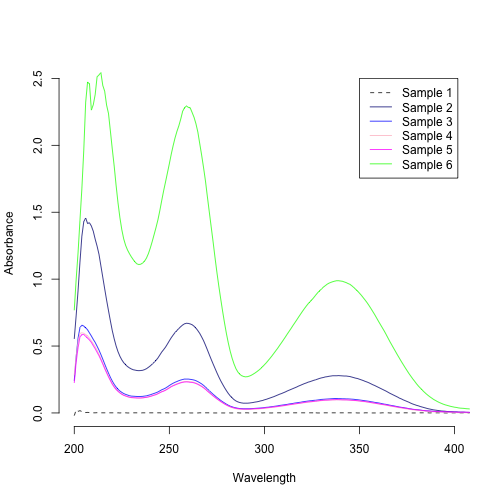
\includegraphics[width=200px]{../resources/absorption_r1_spectrum.png} &
                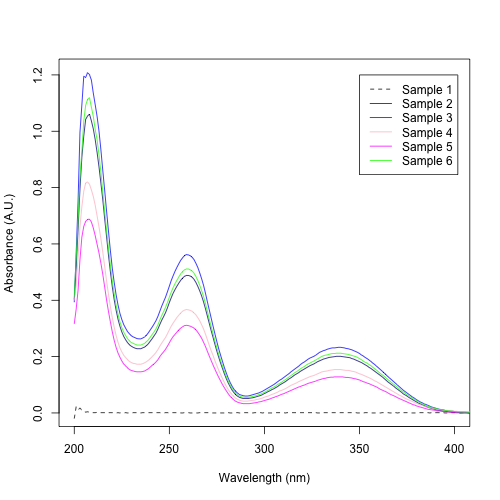
\includegraphics[width=200px]{../resources/absorption_r2_spectrum.png} \\
                (a) & (b)\\
            \end{tabular}
            \caption{Absorbance spectrum of NADH for different concentrations}
            \label{fig:abs_spectrum}
        \end{figure}

        \subsection*{Analysis}
            \begin{figure}[H]
                \centering
                \begin{tabular}{cc}
                    
\includegraphics[width=200px]{../resources/absorption_r1_340.png} &
                    
\includegraphics[width=200px]{../resources/absorption_r2_340.png} \\
                    (a) & (b)\\
                \end{tabular}
                \caption{Absorbance at 340nm for different concentrations}
                \label{fig:abs_340}
            \end{figure}
    \pagebreak

\end{document}